\chapter{Literature Review}
\label{ch:lit-review}

The literature review is broken into five sections.  I first examine
what a season \emph{is}; how they are defined and why this matters.
I then explain tropical seasonality as understood by climate scientists,
before giving an academic perspective on Indigenous Knowledge.
I cover the literature on Indigenous seasons with a particular
focus on Northern Australia, and finally identify a broad gap in the
literature which this thesis begins to fill.



\section{What are Seasons?}

TODO: Relationship to phenology and historical climate change

I canvas the concrete applications of 
seasonality and the potential benefits of this research.

what constitutes a season (weather, time, or ecology?),
and the role of phenology in determining seasons as a link in to Indigenous 
calendars.

Seasons – specifically what makes something a season – is obviously key.  
Passage of time is one simplistic definition.  Others look at meteorology, or 
at ecology... which ties into phenology, which leads us back to Indigenous
Seasons in the next subsection!


Growing use of phenology in description of climate and climate change; similar 
use in IEK

Phenology is the study of timing in ecological events, usually associated with 
the first such event in a given year – such as the date of bloom for flowering 
plants, or the first sighting of migratory species.  Plant phenology is so 
closely associated with temperature (especially in temperate regions) or water 
availability (in arid regions) as to be a common proxy for measurement of such 
variables (REF).

Some phenological records in Europe go back centuries, and recent analyses show 
their significant value in understanding past climate conditions.
\citet{allstadt2015} look at leaf-out phenology as a definition of spring 
in the USA.  \citet{menzel2006} examine changes in butterfly presence in the
UK under observed climate change.




\section{The Tropical Climate}

Tropical seasonality, including monsoon and ENSO

Still too narrow; needs a section on the climatology of the region (a pag-ish),
section includes map of ITCZ and intro to monsoon systems; lays out simple scientific view.
(REF - Cook and Hedergan (sp?) on monsoon onset, Int. J. of Climatology).

Need to cover why seasons matter (reinforcing introduction); should tie
closely into section on tropical climatology (Put climograph from results here instead?)



\autoref{fig:galiwinku-climograph} is a typical example of tropical seasons.
To see the more nuanced patterns described by Indigenous seasons, daily data is required.

\begin{figure}[h]
    \centering
    \includegraphics[width=\textwidth]{galiwinku/climograph.pdf}
    \caption[Monthly Climograph for Galiwinku]{
        Monthly summary of climate statistics at Galiwinku, showing the per-day
        mean for each month.  Rainfall (vertical bars), maximum temperature
        (solid line), minimum temperature (dashed line), and  dewpoint
        temperature (dotted line).}
    \label{fig:galiwinku-climograph}
\end{figure}


\section{Indigenous Knowledge}

There are a variety of terms used in the literature to describe Indigenous 
ecological knowledge systems:  \citet{clarke2009} refers to `land-based knowledge', 
\citet{petheram2010} and \citet{turner2009} use `traditional ecological 
knowledge', while \citet{cochran2015} simply use `indigenous knowledge'.  
\citet{berkes2012} defines Indigenous Ecological Knowledge (IEK) as ``a cumulative 
body of knowledge, practice and belief, evolving by adaptive processes and 
handed down through generations by cultural transmission''.  I prefer 
`Indigenous knowledge' to emphasise that ecology is not the only subject of 
Indigenous knowledge – for example, seasonal calendars often have cultural and 
economic as well as ecological importance.

WHY IS THIS KNOWLEDGE IMPORTANT - expands to why my research matters.
(related to fine-scale timing, as the nuance matters in land and NRM)

There is a growing recognition among ecologists, natural resource managers, and 
scholars worldwide that Indigenous peoples hold important knowledge about the 
natural environment. The literature on IEK is well-established and vibrant.  In 
Australia and around the world, the value of Indigenous knowledge is recognised 
in areas as diverse as climate change and sustainability assessment
\citep[eg.][]{cochran2015}, holistic fire management \citep[eg.][]{clarke2009,price2012}, 
customary economic activities including aquaculture \citep{woodward2012a}, and 
natural resource management \citep[eg.][]{prober2011}.  The \textit{Environment 
Protection and Biodiversity Conservation Act 1999} suggests taking `a 
partnership approach to environmental protection and biodiversity conservation'
\citep{ens2012}, which is increasingly common at local and state levels.  

\citet{turner2009} distinguish Indigenous knowledge systems from `objective' 
scientific knowledge on the basis that Indigenous knowledge of practical 
matters is value-laden and observations or experience are tangled with beliefs, 
philosophy, law, and spirituality.  \citet{green2010a} and \citet{clarke2009} 
demonstrate the use of Indigenous phenological and climate knowledge to improve 
western scientific understanding of past and future climates.
EXPAND THIS PARA, see also recent Woodward paper.

This literature provides a rich context for synthesis of indigenous knowledge 
and western climate science to investigate Australian seasonality.
TO WHAT END?



\subsection{Two-ways research}
Broaden approach; not just two-ways – read other research methodology and 
situate work.  Really really need to do this.

Around the world, and more recently in Australia, there has been growing 
interest in `two-ways' research \citep{turner2009,prober2011}, 
which \blockquote{uses combinations of Indigenous and non-Indigenous knowledge and 
methods, and with the involvement of both Indigenous and non-Indigenous people 
towards a common goal} \citep{ens2014}.  

However, working across knowledge systems can be difficult for both Indigenous 
and non-Indigenous people, and often challenges institutions and research 
funding bodies to invest substantial time and resources in relationship-
building with uncertain outcomes.  The Ngan'gi Seasons Calendar emphasises 
ecological events and customary activities for each season above the timing and 
meteorological conditions.  Produced in collaboration between Ngan'gi knowledge 
holders and the CSIRO, `success' required a long-term commitment to work in 
remote areas on the Daly River, a high degree of risk tolerance in 
research funding, and many years work building solid relationships \citep{woodward2010}.

TODO - A bit thin; expand benefits and value of knowledge

When \citet{petheram2010} investigated perspectives on climate change 
adaptation in NE Arnhem Land; the community engaged in terms of resilience to 
existing issues rather than adaptation to climate change, challenging the basis 
of their research.  With severe problems related to poor housing, drug abuse, 
and extensive mining land degradation, climate change is of little concern to 
participants who mostly attribute `strange changes' to local environmental 
damage \citep{green2010a}.




\section{Australian Indigenous Seasons}

Summarise, compare and contrast Indigenous seasons literature.
Indigenous knowledge of phenology stretches back millennia – and much is 
encoded in the seasonal calendars and traditions.\\


Documenting indigenous calendars – see eg \textit{Man of All Seasons} \citep{davis1989},
the Indigenous Weather Knowledge project \citet{BOM-iwk},
or CSIRO’s Tropical Rivers and Coastal Knowledge (TRaCK) program \citep{CSIROcals,oconnor2010}.


This section is not finished, but you get a pretty good idea where it's 
going.  Mainly it needs to be fleshed out with examples, references, etc. 

Indigenous seasonal calendars are qualitatively different to the European 
system, which was marked by lunar and later solar cycles.  By contrast, 
Australian indigenous seasonal calendars are defined by climatic and ecological 
cycles, with all the sensitivity to local context and variation between years 
that implies.

For practical use, a local and long-tested seasonal calendar is likely to have 
substantial advantages over one imported from Europe – at least for 
applications which depend on an understanding of Australia's environment, such 
as fire or natural resource management.

European seasons are adapted for agriculture in temperate regions.

Australian Indigenous calendars are generally adapted to a hunter-gatherer, 
more mobile lifestyle.  They also must cope with a far higher degree of 
interannual variation and offer more complex detail to be as useful.  It's no 
coincidence that the calendar is based directly on the important climate 
variables and marked by ecological events:  instead of ``the Wet is usually a 
good time for these foods'', the knowledge is more like ``after the first big 
storm (which marks this season), all the fish gather in these places''.



TODO - survey the general and specific projects documenting Australian Indigenous
seasons, and comment on each.

General - BOM-IWK, CSIRO TRaCK project, CDU?.  For Yolngu seasons, Davis, Atlas, and I.

% commented out due to large file size and slow rendering.
%\begin{landscape}
%\begin{figure}[p]
%    \centering
%    \includegraphics[width=\paperwidth]{TiwiSeasons.pdf}
%    \caption[The Tiwi Seasons Calendar \citep{CSIROcals}]{
%        The Tiwi Seasons Calendar \citep{CSIROcals}.
%        This calendar shows month of year in the outermost ring,
%        then three `major' Tiwi seasons recognised by weather.
%        Note that \textit{Kumunupunari} does not have a sharp boundary with \textit{Tiyari}!
%        Within this ring are smaller seasons, recognised by weather
%        or ecological events and associated with particular activities.
%        This format is designed for the circle to rotate, encouraging interaction or observation.
%        }
%    \label{fig:tiwi-seasons}
%\end{figure}
%\end{landscape}


\begin{figure}[h]
    \centering
    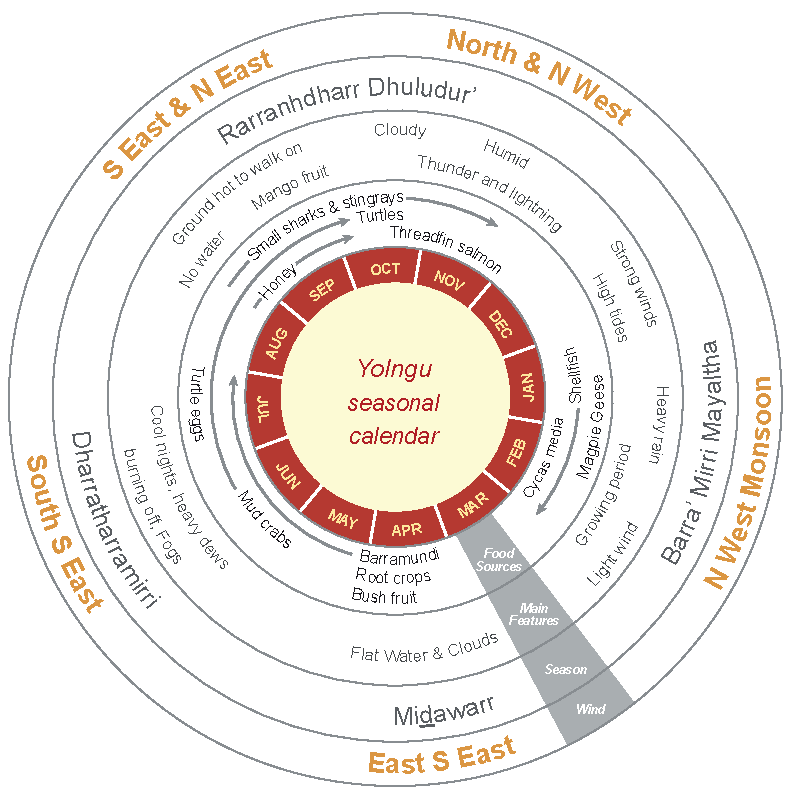
\includegraphics[width=0.7\textwidth]{davis1989_yolngu_seasons.pdf}
    \caption[Conceptual Yolngu seasonal calendar \citep{davis1989}]{
        Conceptual Yolngu seasonal calendar, redrawn from \citet{davis1989}.
        TODO - cite page number
        
        This calendar shows a glimpse of the relationships between season,
        prevailing wind, typical conditions, and available foods.
        It also shows typical gregorian months, for non-Indigenous readers.
        }
    \label{fig:yolngu-seasons}
\end{figure}




\section{The Gap in the Literature}

There is a paucity of research which treats indigenous knowledge
as a \emph{framework for} research, instead of an \emph{object of} research.
This gap in the literature persists despite the novely and potential value
of combining Indigenous seasonal knowledge with quantitative climate science.

After -detailed search strategy-, I was unable to identify any studies which 
quantified indigenous Australian seasons.  PARA ON LIT SEARCH STRATEGY


MOVE TO RESULTS: none of the participants I interviewed were aware of
attempts to quantify indigenous seasons, and several made spontaneous
comments as to the novelty of this approach.



\section{Methods}


\subsection{Research with Indigenous People}

VERY INCOMPLETE

Rather than structured interviews or a written survey, I conduct minimally-
directed conversations with research participants.  Bringing avoidable 
paperwork to an indigenous community is generally not culturally appropriate, 
as it can devolve into mutual frustration rather than mutual learning.  An 
assumption of literacy may exclude potential participants where English is 
often a fourth (or sixth, or later!) language.

Calendars and seasons are a topic which is not usually secret business, though 
there may be particular sacred topics associated with them.  Especially with an 
explicit invitation to come and learn, there is little risk of inappropriate 
sharing of information.


Relationships are a key part of cross-cultural research.  See Sue Smith, as 
Sean has mentioned.

This collaborative and cross-cultural approach has been and will be a 
significant influence on the direction of the research. (explore it more then)



\subsection{Quantitative handling of seasons}

Some stuff will move here.


